\subsection{Stability}
\label{sec:dcqcn_stability}

\begin{figure*}[t]
\center
\subfigure[Default parameters ($R_{AI}=40Mbps$, $K_{max}=200KB$).]
{
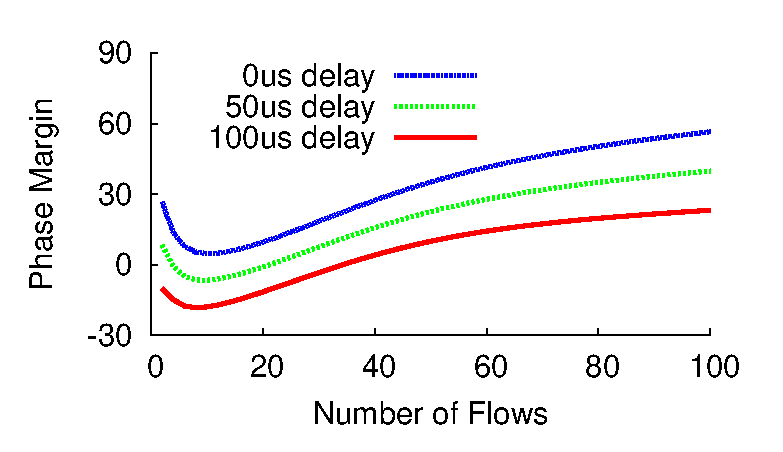
\includegraphics[width=0.3\textwidth]{figures/dcqcn_stability.eps}
\label{fig:dcqcn_stability_default}
}
\subfigure[$R_{AI}=10Mbps$.]
{
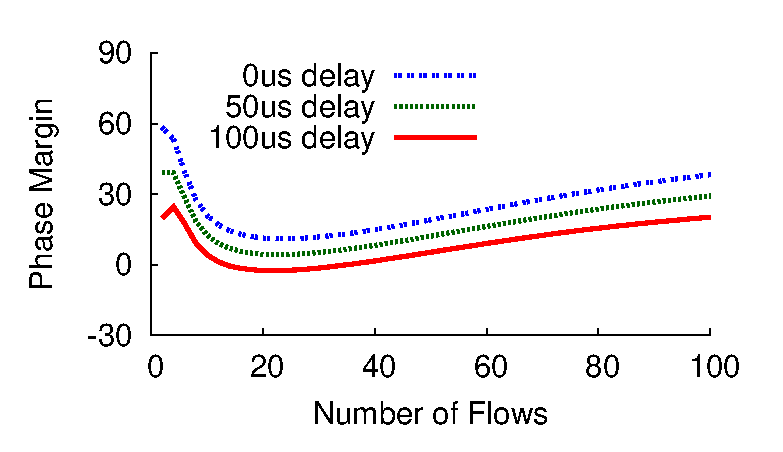
\includegraphics[width=0.3\textwidth]{figures/dcqcn_stability_rai.eps}
\label{fig:dcqcn_stability_rai}
}
\subfigure[$R_{AI}=10Mbps$ and $K_{max}=1000KB$.]
{
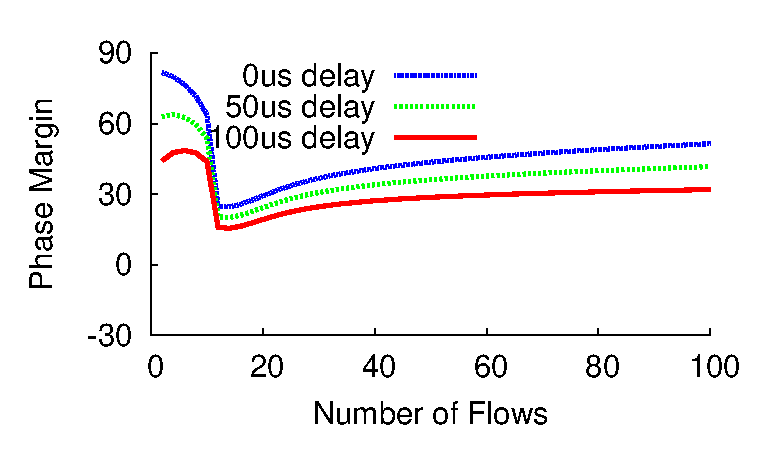
\includegraphics[width=0.3\textwidth]{figures/dcqcn_stability_rai_kmax.eps}
\label{fig:dcqcn_stability_rai_kmax}
}
\caption{DCQCN stability}
\label{fig:dcqcn_stability}
\end{figure*}
To analyze stability, we first obtain the fixed point of the system, and then
linearize the model around the fixed point. We analyze the linearized model for
stability using classical frequency domain techniques~\cite{controltheory}.  

\begin{thm}[DCQCN's unique fixed point]
A unique fixed point of queue length exists for DCQCN. 
\end{thm}
\begin{proof}
By setting the left-hand side of Equation~\ref{eq:q} to 0,
it is easy to see that any fixed points of the DCQCN (if they exist) must
satisfy:
\begin{equation}
\small
\sum\limits_{i = 1}^N {R_C^{(i)}(t)} = C
\label{eq:fixedrc}
\end{equation}
At any of the fixed points, we assume the value of $p$ is $p^*$, which is shared
by all flows. The queue length and per-flow $\alpha^{(i)}$ at the fixed points
are determined by Equation~\ref{eq:mark} and \ref{eq:alpha}:
\begin{equation}
\small
{q^*} = \frac{{{p^*}}}{{{p_{max}}}}\left( {{K_{max}} - {K_{min}}} \right) + {K_{min}}
\end{equation}
\begin{equation}
\small
\alpha^{(i)*}  = 1 - {(1 - p^*)^{{\tau '}R_C^{(i)*}}}
\end{equation}
Next, we show that $p^*$ exists and is uniquely determined by $R_C^{(i)*}$ in
the DCQCN model. Combining Equation~\ref{eq:rt} and \ref{eq:rc}, 
we eliminate the variable $R_T^{(i)*}$. After simplification, we see that the value 
of $p^*$ is determined by:
\begin{equation}
\small
\frac{{{a^2}\alpha^{(i)*} }}{{(b + d)(c + e)}} = {\tau ^2}{R_{AI}}R_C^{(i)*}
\label{eq:p_fixed}
\end{equation}
Where we denote $a, b, c, d, e$ as follows:
\begin{equation}
\small
\begin{array}{l}
a = 1 - {(1 - p^*)^{\tau {R_C^{(i)*}}}},b = \frac{{p^*}}{{{{(1 - p^*)}^{ - B}} - 1}},c = \frac{{{{(1 - p^*)}^{FB}}p^*}}{{{{(1 - p^*)}^{ - B}} - 1}},\\
d = \frac{{p^*}}{{{{(1 - p^*)}^{ - T{R_C^{(i)*}}}} - 1}},e = \frac{{{{(1 - p^*)}^{FT{R_C^{(i)*}}}}p^*}}{{{{(1 - p^*)}^{ - T{R_C^{(i)*}}}} - 1}}
\end{array}
\end{equation}
%at the fixed point,
%we get the two forms of $R_T^{(i)*}$, respectively:
%\begin{equation}
%\small
%{R_T^{(i)*}} = R_C^{(i)*} + \frac{{a\alpha^{(i)*} }}{{(b + d)\tau }}
%\end{equation}
%\begin{equation}
%\small
%{R_T^{(i)*}} = R_C^{(i)*}\left( {1 + \frac{{(c + e)\tau {R_{AI}}}}{a}} \right)
%\end{equation}
%Combining the two forms of $R_T^{(i)*}$, we see that the value of $p^*$ is determined by:
The LHS of Equation (\ref{eq:p_fixed}) is a monotonic function of $p$ when $p \in [0,1]$.
Furthermore, when $p = 0$, the LHS is smaller than RHS, and vice versa when $p =
1$. Thus DCQCN has a unique fixed point of marking probability $p^*$, leading to
a unique fixed point of queue length $q^*$.
\end{proof}

Next we approximate the value of $p^*$. Numerical analysis shows that $p^*$ is 
typically very close to 0. Therefore, we approximate the LHS using Taylor series around $p=0$.
%\begin{equation}
%\small
%\frac{{{a^2}\alpha }}{{(b + d)(c + e)}} = \frac{{(R_C^{(i)*})^3{\tau ^2}\tau '}}{{{{\left( {\frac{1}{B} + \frac{1}{{TR_C^{(i)*}}}} \right)}^2}}}{p^3} + O\left( {{p^4}} \right)
%\end{equation}
After omitting the $O(p^4)$ term in the Taylor series, we have:
\begin{equation}
\small
{p^*} = \sqrt[3]{{\frac{{{R_{AI}}}}{{{\tau '}(R_C^{(i)*})^2}}{{\left( {\frac{1}{B} + \frac{1}{TR_C^{(i)*}}} \right)}^2}}}
\label{eq:fixedp}
\end{equation}
With this estimation, we see that $p^*$ uniquely determine $R_C^{(i)*}$. 
Since $p^*$ is shared by all flows $i$, $i = 1, 2, ..., N$, we have:\footnote{In 
Section~\ref{sec:dcqcn_convergence}, we show a more rigorous proof that all flows
converge the the same rate.}
\begin{equation}
\small
R_C^{(1)*} = R_C^{(2)*} = ... = R_C^{(N)*}
\end{equation}
Combining this with Equation~\ref{eq:fixedrc}, proves that at the fixed point, $R_C^{(i)*} = \frac{C}{N}$, 
$i = 1, 2, ..., N$.

\para{Stability analysis.} 
We test the system against {\em Bode Stability Criteria}~\cite{controltheory}. 
More details can be found in~\cite{fullpaper},
while the final results are shown in
Figure~\ref{fig:dcqcn_stability}.  The degree of stability is shown as {\em
Phase Margin}. The system is stable when its {\em Phase Margin} is larger than
0, and the larger {\em Phase Margin} means the system is more stable.

We analyze DCQCN stability in different conditions, particularly with different
control signal delays (propagation delay plus queuing delay in practice), and
different number of flows. An ideal protocol should be tolerant with large delay
and scalable to any number of flows. As Figure~\ref{fig:dcqcn_stability} shows,
DCQCN, with default parameters, is mostly stable. In most cases, the phase
margin is larger than 0.

\begin{figure*}[t]
\centering
\mbox{
\begin{minipage}{0.66\textwidth}
\subfigure[] {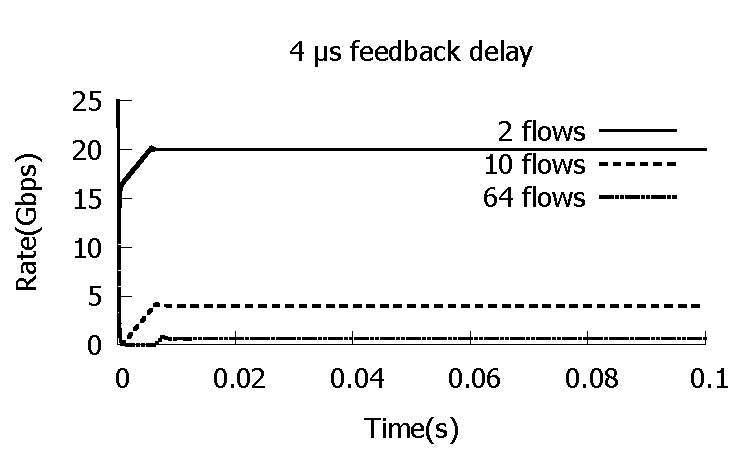
\includegraphics[width=0.49\columnwidth]{figures/stable_rate_4.pdf}}
\subfigure[] {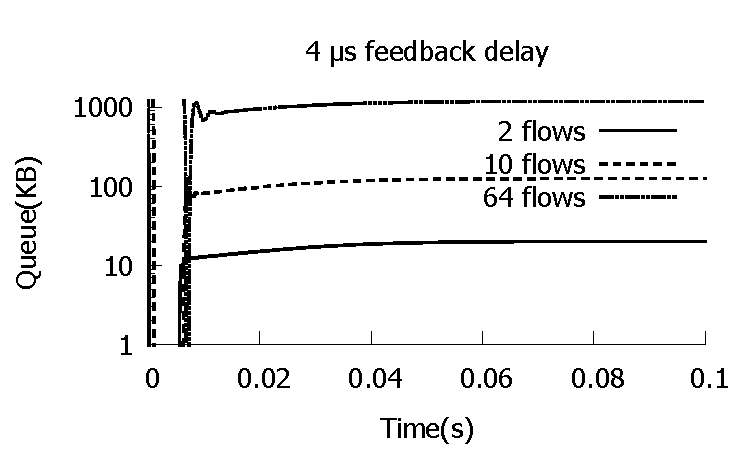
\includegraphics[width=0.49\columnwidth]{figures/stable_q_4.pdf}}
\subfigure[] {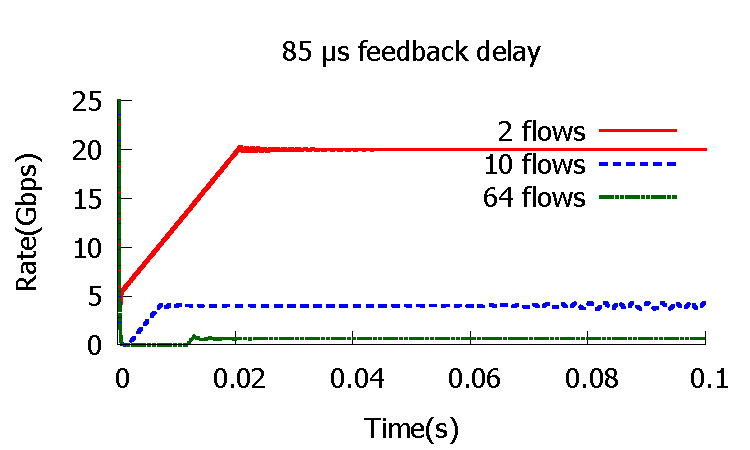
\includegraphics[width=0.49\columnwidth]{figures/stable_rate_85.pdf}}
\subfigure[] {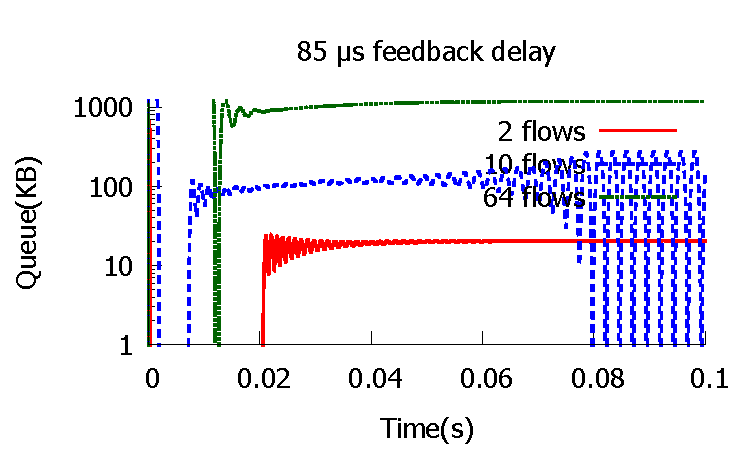
\includegraphics[width=0.49\columnwidth]{figures/stable_q_85.pdf}}
\caption{Impact of delay and number of flows on DCQCN stability}
\label{fig:dcqcn_unstable}
\end{minipage}

\begin{minipage}{0.33\textwidth}
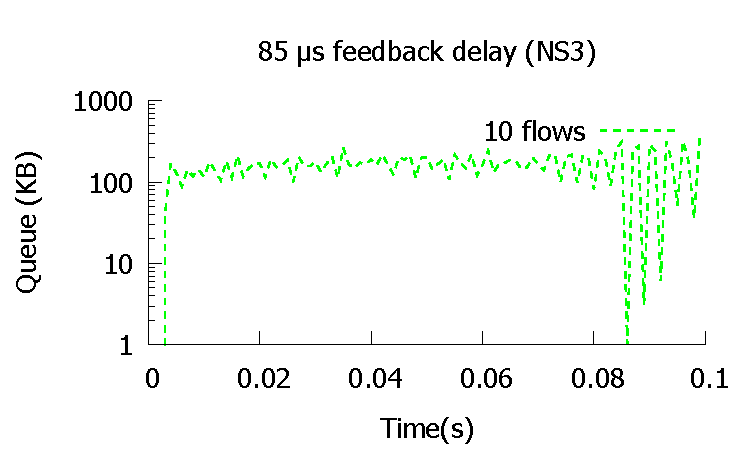
\includegraphics[width=0.99\columnwidth]{figures/stable_queue_85_ns.pdf}
%\vspace{-2em}
\caption{NS simulations confirm lack of stability}
\label{fig:dcqcn_unstable_ns}

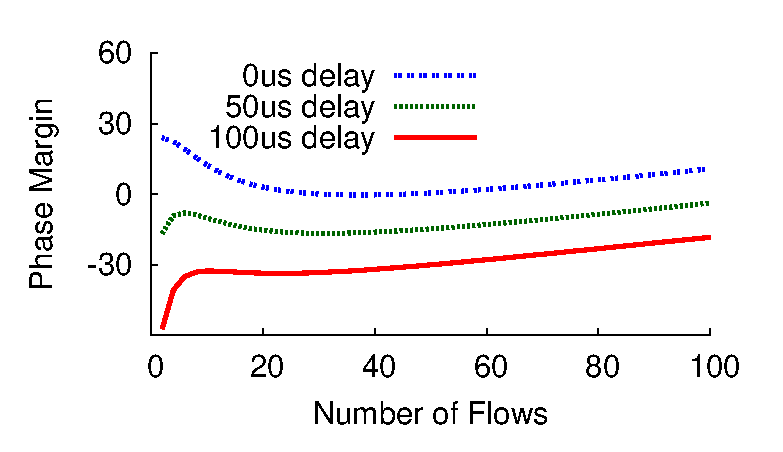
\includegraphics[width=0.99\columnwidth]{figures/dcqcn_stability_100gbps.eps}
\caption{DCQCN stability with 100Gbps}
\label{fig:dcqcn_100gbps}
\end{minipage}
}
\end{figure*}

\begin{figure}[t]
\centering
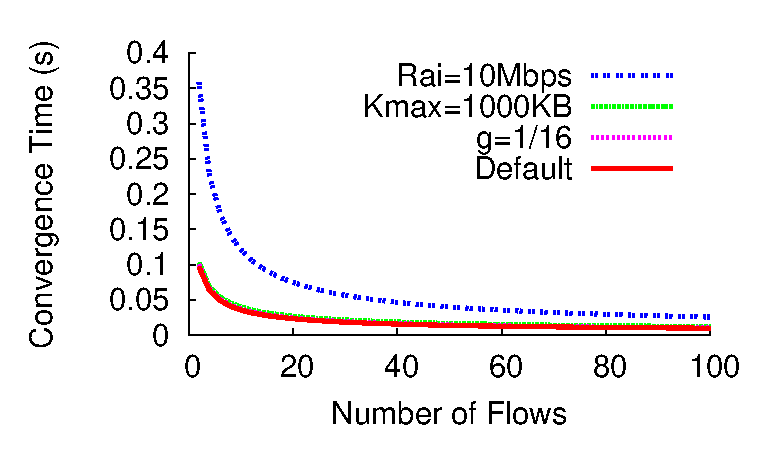
\includegraphics[width=0.33\textwidth]{figures/dcqcn_convergence_time.eps}
\vspace{-1em}
\caption{Upper bound on DCQCN convergence time under conservative assumptions}
\vspace{-1em}
\label{fig:dcqcn_convergence_time}
\end{figure}

%\begin{figure}[t]
%\center
%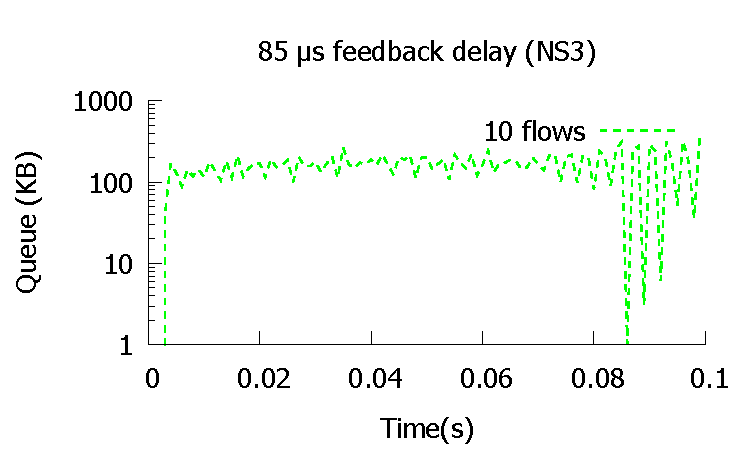
\includegraphics[width=0.4\textwidth]{figures/stable_queue_85_ns.pdf}
%\caption{NS simulations confirm lack of stability}
%\label{fig:dcqcn_unstable_ns}
%\end{figure}

Curiously, unlike TCP, the relationship between number of flows and the phase
margin is non-monotonic. When the delay is large, {\em e.g., 100$\mu$s}, the
phase margin dips below zero for certain number of flows, before rising again.
For the set of parameters we have chosen, the system can be unstable with 10
flows at high feedback delays.  DCQCN is increasingly stable with larger number
of flows, which means good scalability. This point is further illustrated in the
fluid model results shown Figure~\ref{fig:dcqcn_unstable}. When the feedback
delay is small (4 $\mu$s), DCQCN is stable - flow rates, and queue length
quickly\footnote{Remember that DCQCN flows always start at line rate.}
stabilizes regardless of the number of flows. However, when the delay is large
(85$\mu$s), the protocol is unstable for 10 flows. It is, however, stable for 2
and 64 flows. Figure~\ref{fig:dcqcn_unstable_ns} confirms that we observe the
same instability in packet-level simulations.

While this problem may not be particularly serious in practice, it can be easily 
fixed by tuning the values of $R_{AI}$ and $K_{max}$.  Smaller $R_{AI}$
means flows increase their rate more gently, and stabilizes the system.
Similarly, larger $K_{max} - K_{min}$ makes rate decreasing more fine grained,
because the perturbation of queue length leads to smaller marking probability
perturbation. We show these trends in Figures \ref{fig:dcqcn_stability_rai} and
\ref{fig:dcqcn_stability_rai_kmax}.  With small $R_{AI}$ and large $K_{max}$,
DCQCN can be always stable even when the control signal delay reaches 100$\mu
s$, which equals to the propagation delay of a $30KM$ cable, or $500KB$ queuing
delay. Such large delays are rare in modern datacenter networks. 

Note that tuning $R_{AI}$ and $K_{max}$ is a trade-off between stability and
latency. Smaller $R_{AI}$ leads to slower ramp-up, while larger $K_{max}$ leads
to larger queue length. In most cases, the default parameters strike a good
enough balance between stability and latency.

\para{Extending to 100Gbps network.}  As the datacenter network fabric is moving
towards 100Gbps bandwidth, we analyze DCQCN stability given $C=100Gbps$. As
shown in Figure~\ref{fig:dcqcn_100gbps}, the default parameters of DCQCN work
reasonably well when the delay is small, {\em e.g.,} close to $0\mu s$.
However, DCQCN on 100Gbps is sensitive to the control loop delay. With
$50\mu s$ and $100\mu s$, the phase marginal decreases much more than in 40Gbps
case and leads to consistent instability.  The methods that stabilize the 40Gbps
system, like tuning down $R_{AI}$ and tuning up $K_{max}$, are also effective in
100Gbps system. Though we verified that tuning $R_{AI}$ and $K_{max}$
can help stabilize DCQCN at 100Gbps at the price of convergence speed and queue length, 
we believe PI controller is a more favorable option.
